% vim: filetype=tex spell

%define some math commands
\newcommand{\vect}[1]{\overrightarrow{#1}}
\newcommand{\cross}[0]{\times}
\newcommand{\matt}[1]{\boldsymbol{#1}}
\newcommand{\transpose}{^T}
\newcommand{\unit}[1]{\, \mathrm{#1}}

%highlight future work
\newcommand{\future}[1]{{\color{red}\itshape#1}}

\pgfdeclareshape{inshape}
{%
  % All anchors are taken from the 'rectangle' shape:
  \inheritsavedanchors[from={rectangle}]%
  \inheritanchor[from={rectangle}]{center}%
  \inheritanchor[from={rectangle}]{north}%
  \inheritanchor[from={rectangle}]{south}%
  \inheritanchor[from={rectangle}]{west}%
  \inheritanchor[from={rectangle}]{east}%
  \inheritanchorborder[from={rectangle}]%
  %
  % Only the background path is different
  %
  \backgroundpath{%
    % First the existing 'circle' code:
    \pgfmathsetlength{\pgf@xb}{\pgfkeysvalueof{/pgf/outer xsep}}%
    \pgfmathsetlength{\pgf@yb}{\pgfkeysvalueof{/pgf/outer ysep}}%
    \ifdim\pgf@xb<\pgf@yb%
      \advance\pgfutil@tempdima by-\pgf@yb%
    \else%
      \advance\pgfutil@tempdima  by-\pgf@xb%
    \fi%
    \pgfpathcircle{\centerpoint}{\pgfutil@tempdima}%
    %
    % Now the | and -- lines:
    \pgfmoveto{\pgfpointadd{\centerpoint}{\pgfpoint{0pt}{\pgfutil@tempdima}}}%
    \pgflineto{\pgfpointadd{\centerpoint}{\pgfpoint{0pt}{-\pgfutil@tempdima}}}%
    \pgfmoveto{\pgfpointadd{\centerpoint}{\pgfpoint{\pgfutil@tempdima}{0pt}}}%
    \pgflineto{\pgfpointadd{\centerpoint}{\pgfpoint{-\pgfutil@tempdima}{0pt}}}%
  }%
}

%set default arrows to stealth
\tikzset{>=latex}
% Define block styles
\tikzstyle{decision} = [diamond, draw, fill=blue!20, text width=4.5em, text badly centered, inner sep=0pt]
\tikzstyle{block} = [rectangle, draw, fill=blue!20, text width=5em, text centered, rounded corners, minimum height=4em]
\tikzstyle{bigblock} = [rectangle, draw, fill=blue!20,rounded corners, minimum height=4em]
\tikzstyle{input} = [rectangle, draw, fill=green!20, text width=5em, text centered, rounded corners, minimum height=4em]
%\tikzstyle{input} = [inshape, draw, fill=green!20, text width=5em, text centered, minimum height=4em]

\tikzstyle{oppr} = [draw, circle,fill=blue!20,minimum height=2em]
\tikzstyle{cloud} = [draw, ellipse,fill=red!20, node distance=3cm,minimum height=2em]
%connections styles for flow charts
\tikzstyle{line} = [draw]
\tikzstyle{conn} = [draw,->]
\tikzstyle{phconn} = [draw,->,dashed]
%connection styles for block diagrams
\tikzstyle{bidr} = [draw,<->]
%\tikzstyle{flow} = [draw,--,decorate,decoration=triangles]
\tikzstyle{flow} = [draw,%
          decoration={%
            markings,%
            mark=at position 0.65 with {\arrow[scale=2]{stealth}},
          },postaction=decorate]
          
%hardware block diagram styles
\tikzstyle{powerL} = [draw,color=red!80,thick,line width=0.5mm]
\tikzstyle{powerB} = [->,ultra thick,draw,color=red!50,line width=0.5mm]
\tikzstyle{dataL} = [draw,color=blue,line width=0.5mm]
\tikzstyle{commandL} = [draw,color=green]
\tikzstyle{power} = [rectangle, draw, fill=red!80!black, text width=5em, text centered, minimum height=4em,on chain]
\tikzstyle{prog} = [rectangle, draw=red!30, fill=red!20,text width=5em,text centered,on chain,node distance=1cm]
\tikzstyle{perif} = [rectangle, draw=green!80, fill=green!40,text centered,on chain]
\tikzstyle{hardware} = [rectangle, draw, fill=blue!20, text width=5em, text centered,minimum height=4em,on chain]
\tikzstyle{CPU} = [draw=black,fill=blue!5,inner sep=0]
\tikzstyle{Bus} = [line width=3mm,draw=blue,arrows={Latex[length=3mm,width=7mm]-Latex[length=3mm,width=7mm]}]
\tikzstyle{PCB} = [rectangle,draw=black,inner sep=5mm]



%point used as a dummy node for complicated arrows
\tikzstyle{point} = [circle,inner sep=0pt,minimum size=0pt,fill=none,node distance = 0.5cm]
%\tikzstyle{point} = [circle,inner sep=0pt,minimum size=2pt,fill=red,node distance = 0.5cm]     %alternate point for debugging

%style for annotating fiugres
\tikzstyle{na} = [baseline=-.5ex,remember picture]

%name of MATLAB
\newcommand{\matlab}{MATLAB\xspace}

%draw cubesat with axes
\newcommand{\cubesat}[2]{
    \draw (#1:#2) node{\pgftext[rotate=#1]{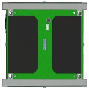
\includegraphics[height=\ARCheight]{cube-icon}}};
    \draw[->,cyan,thick] (#1:#2) -- +(#1+90:\axlen);
    \draw (#1:#2) ++(#1+90:\axlen) node[rotate=#1-90,anchor=south west] {\tiny +Y};
    \draw[->,red,thick] (#1:#2) -- +(#1:\axlen);
    \draw (#1:#2) ++(#1:\axlen) node[rotate=#1-90,anchor=north west] {\tiny -Z};
}

%styles for bias modes
\tikzstyle fieldarrow=[arrows={-Latex[color=blue,fill=red,length=3mm,width=1.5mm]}]  %field arrow style
\tikzstyle bias=[<->,YellowOrange,very thick]                                        %bias arrows style

%field lines for winplace figure
\tikzstyle field=[color=blue,thick,postaction={decorate,decoration={markings,mark=at position .35 with {\arrowreversed[thin]{Latex[length=8mm,width=3mm,fill=red]}}}}]

%rotation arrow style for winplace figure
\tikzstyle motion=[->,Plum,very thick]

%draw magnet
\newcommand{\magnet}{
    %draw magnet
    \fill[color=white] (0.25,0.5) rectangle (-0.25,0);
    \fill[color=red] (0.25,0) rectangle (-0.25,-0.5);
    \draw[color=red] (0, 0.2) node {S};
    \draw[color=white] (0,-0.2) node {N};
    \draw[color=black] (0.25,0.5) rectangle (-0.25,-0.5);
}

%draw magnetic field lines
\newcommand{\fieldlines}{
    \begin{scope}
        \clip (0,0) circle (3cm);

        % Computes a point on a field line given r and t
        \newcommand{\fieldlinecurve}[2]{%
            {(pow(##1,2))*(3*cos(##2)+cos(3*(##2)))*0.7}, {(pow(##1,2))*(sin(##2)+sin(3*(##2)))}%
        }

        \foreach \r in {0.85,0.98,1.3,1.8} {
            \draw[color=blue,smooth,variable=\t, samples at={0,-5,-10,...,-360}] plot (\fieldlinecurve{\r}{\t});
        }

        \draw[fieldarrow] (\fieldlinecurve{0.85}{17}) -- (\fieldlinecurve{0.85}{23});
        \draw[fieldarrow] (\fieldlinecurve{0.98}{23}) -- (\fieldlinecurve{0.98}{28});
        \draw[fieldarrow] (\fieldlinecurve{1.3}{50}) -- (\fieldlinecurve{1.3}{52});
        \draw[fieldarrow] (\fieldlinecurve{1.8}{65}) -- (\fieldlinecurve{1.8}{65.5});

        \draw[fieldarrow] (\fieldlinecurve{0.85}{-23}) -- (\fieldlinecurve{0.85}{-17});
        \draw[fieldarrow] (\fieldlinecurve{0.98}{-28}) -- (\fieldlinecurve{0.98}{-23});
        \draw[fieldarrow] (\fieldlinecurve{1.3}{-52}) -- (\fieldlinecurve{1.3}{-50});
        \draw[fieldarrow] (\fieldlinecurve{1.8}{-65.5}) -- (\fieldlinecurve{1.8}{-65});

        \draw[fieldarrow] (\fieldlinecurve{0.85}{180-17}) -- (\fieldlinecurve{0.85}{180-23});
        \draw[fieldarrow] (\fieldlinecurve{0.98}{180-23}) -- (\fieldlinecurve{0.98}{180-28});
        \draw[fieldarrow] (\fieldlinecurve{1.3}{180-50}) -- (\fieldlinecurve{1.3}{180-52});
        \draw[fieldarrow] (\fieldlinecurve{1.8}{180-65}) -- (\fieldlinecurve{1.8}{180-65.5});

        \draw[fieldarrow] (\fieldlinecurve{0.85}{180+23}) -- (\fieldlinecurve{0.85}{180+17});
        \draw[fieldarrow] (\fieldlinecurve{0.98}{180+28}) -- (\fieldlinecurve{0.98}{180+23});
        \draw[fieldarrow] (\fieldlinecurve{1.3}{180+52}) -- (\fieldlinecurve{1.3}{180+50});
        \draw[fieldarrow] (\fieldlinecurve{1.8}{180+65.5}) -- (\fieldlinecurve{1.8}{180+65});
    \end{scope}
}

\newcommand{\lstMat}{
    \lstinline[style=code,language=Matlab]
}



